%%%%%%%%%%%%%%%%%%%%%%%%%%%%%%%%%%%%%%%%%%%%%%%%%%%%%%%%%%%%%%%%%%%%%%%%%%%%%%%%%%
\begin{frame}[fragile]\frametitle{}
\begin{center}
{\Large Reasoning Concepts}

{\tiny (Ref: Reasoning LLMs With a deep dive into DeepSeek-R1 by Dr. Nimrita Koul and more)}

\end{center}


\end{frame}


%%%%%%%%%%%%%%%%%%%%%%%%%%%%%%%%%%%%%%%%%%%%%%%%%%%%%%%%%%%%%%%%%%%%%%%%%%%%%%%%%%
\begin{frame}[fragile]{What is Reasoning?}
    \begin{itemize}
        \item Reasoning is the ability to draw conclusions based on facts, rules or evidence
		\item Types:
			    \begin{itemize}
				\item  Deductive: ``All humans are mortals, I am a human, so I am mortal. ''
				\item  Inductive: Inferring general patterns from specific examples. `` The sun has risen in the east every day I have observed. The sun will rise in the east tomorrow as well. ''
				\item  Abductive: Making educated guesses e.g. diagnosis from symptoms.
				\item  Probabilistic: Bayesian Inference.
			\end{itemize}
    \end{itemize}
\end{frame}

%%%%%%%%%%%%%%%%%%%%%%%%%%%%%%%%%%%%%%%%%%%%%%%%%%%%%%%%%%%%%%%%%%%%%%%%%%%%%%%%%%
\begin{frame}[fragile]{What is Logical Reasoning?}
    \begin{block}{Logical Reasoning}
		A farmer is going to the market with a wolf, a goat, 
		and a cabbage. He comes to a river with a small boat 
		that can carry only him and one of the three items at 
		a time. If left alone together, the wolf will eat the goat, 
		and the goat will eat the cabbage. How can the 
		farmer get everything safely across the river?
    \end{block}
\end{frame}

%%%%%%%%%%%%%%%%%%%%%%%%%%%%%%%%%%%%%%%%%%%%%%%%%%%%%%%%%%%%%%%%%%%%%%%%%%%%%%%%%%
\begin{frame}[fragile]{What is Mathematical Reasoning?}
    \begin{block}{Mathematical Reasoning}
		 A shopkeeper sells an item at a 20\% profit. If the 
		cost price of the item is increased by Rs 50 and the 
		selling price remains the same, the profit 
		percentage drops to 10\%. What is the original cost 
		price of the item?
    \end{block}
\end{frame}

%%%%%%%%%%%%%%%%%%%%%%%%%%%%%%%%%%%%%%%%%%%%%%%%%%%%%%%%%%%%%%%%%%%%%%%%%%%%%%%%%%
\begin{frame}[fragile]{What is AI Reasoning?}
    \begin{itemize}
        \item AI Algorithms can reason using strict logic rules (rule-based systems)or using flexible 
pattern recognition from input data (neural networks). 
        \item Reasoning models can accurately solve verifiable tasks—such as math, logic puzzles and coding 
tasks.
        \item Models like Anthropic's Claude 3.7 Sonnet, OpenAI's o1, o3, and DeepSeek's DeepSeek- R1 
are reasoning LLMs. 
        \item Such reasoning LLMs are built by finetuning large base models using Reinforcement Learning.
    \end{itemize}
\end{frame}


%%%%%%%%%%%%%%%%%%%%%%%%%%%%%%%%%%%%%%%%%%%%%%%%%%%%%%%%%%%
\begin{frame}[fragile]\frametitle{What is Train-Time Compute?}

      \begin{itemize}
        \item Train-time compute combines model size, dataset size, and FLOPs.
        \item More pretraining compute typically yields better models.
        \item Dataset tokens and parameters grow with compute budget.
        \item Pretraining data is referred to as the “fossil fuel of AI”.
        \item Fine-tuning compute is also included in train-time compute.
        \item Key focus area to boost LLM performance before 2024.
      \end{itemize}

        \begin{center}
        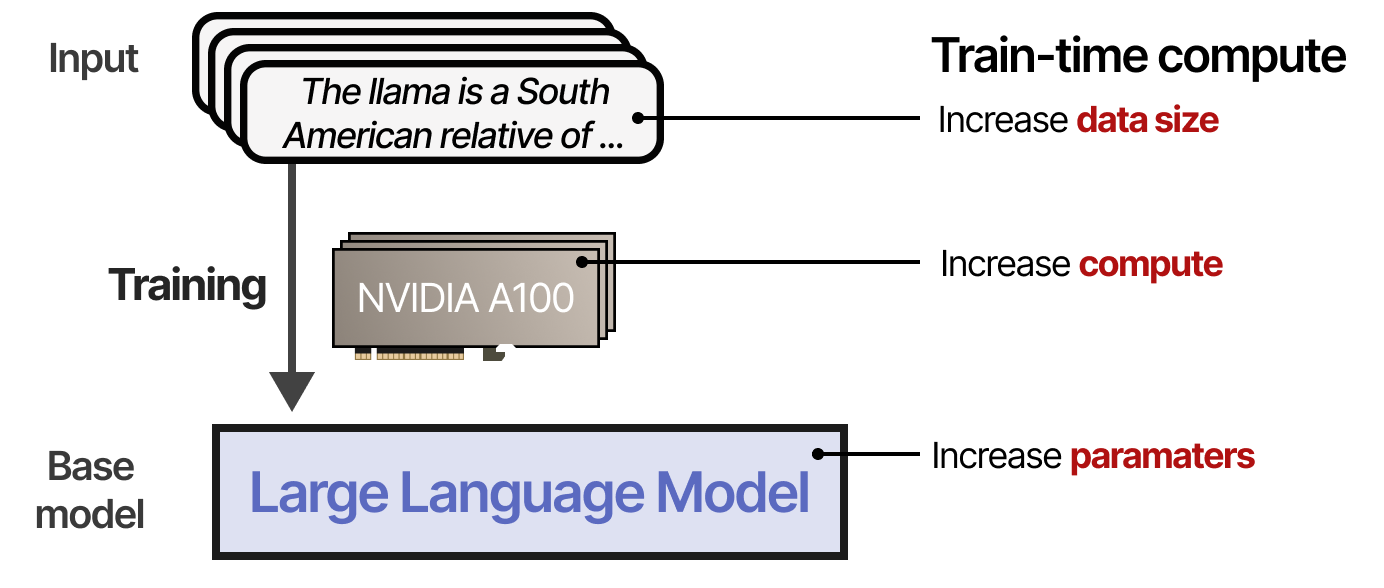
\includegraphics[width=0.6\linewidth,keepaspectratio]{llm243}
		
        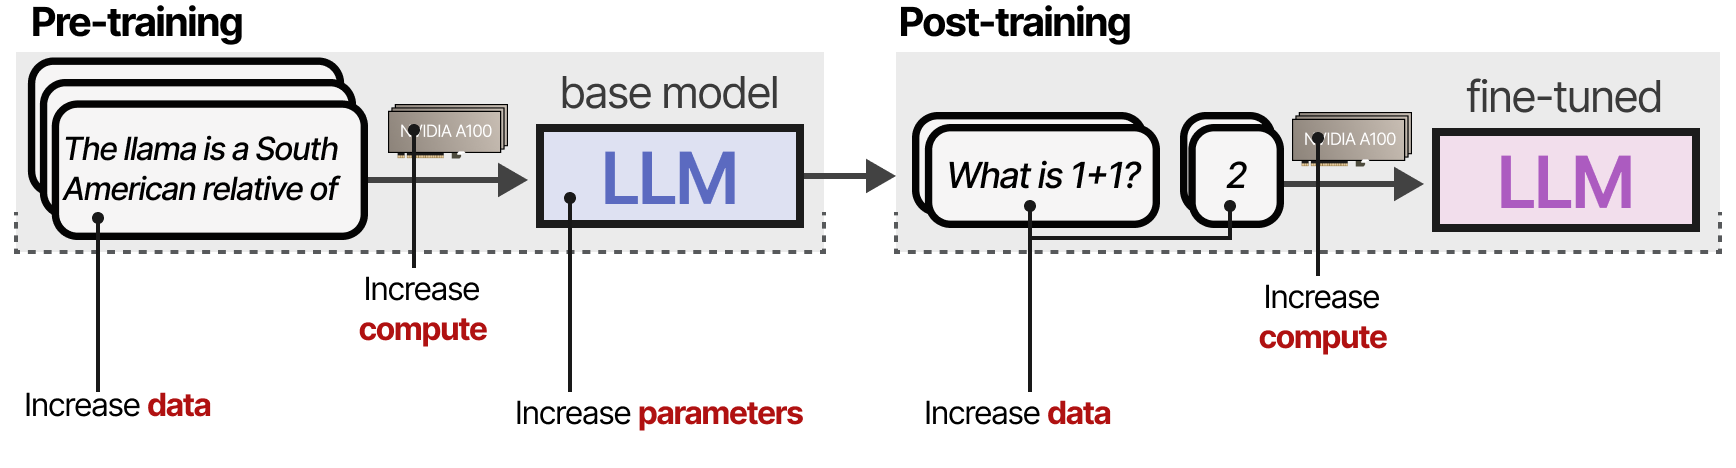
\includegraphics[width=0.6\linewidth,keepaspectratio]{llm244}
		

		{\tiny (Ref: A Visual Guide to Reasoning LLMs - Maarten Grootendorst)}
		
        \end{center}    

\end{frame}

%%%%%%%%%%%%%%%%%%%%%%%%%%%%%%%%%%%%%%%%%%%%%%%%%%%%%%%%%%%
\begin{frame}[fragile]\frametitle{Scaling Laws Overview}

      \begin{itemize}
        \item Scaling laws show how compute affects model performance.
        \item Based on power-law relationships shown in log-log plots.
        \item Kaplan Law: prioritize model size over data for fixed compute.
        \item Chinchilla Law: balance model size and dataset for best results.
        \item All three dimensions—compute, data, parameters—must scale together.
        \item Gains in 2024 showed diminishing returns despite scale increases.
      \end{itemize}

        \begin{center}
        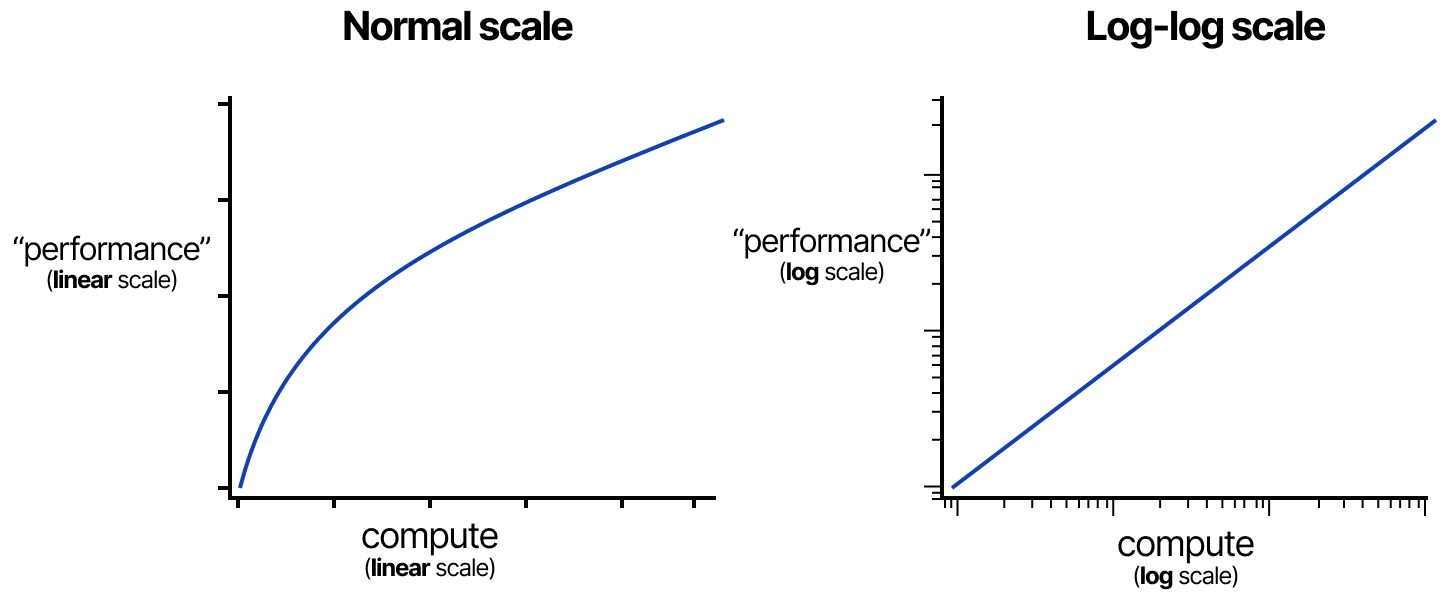
\includegraphics[width=0.8\linewidth,keepaspectratio]{llm245}
		
		{\tiny (Ref: A Visual Guide to Reasoning LLMs - Maarten Grootendorst)}
		
        \end{center}    

\end{frame}

%%%%%%%%%%%%%%%%%%%%%%%%%%%%%%%%%%%%%%%%%%%%%%%%%%%%%%%%%%%
\begin{frame}[fragile]\frametitle{What is Test-Time Compute?}
\begin{columns}
    \begin{column}[T]{0.5\linewidth}
      \begin{itemize}
        \item Test-time compute refers to inference-time resource usage.
        \item Reasoning models use more tokens to "think" during inference.
        \item Allows deeper, structured answers vs. direct output.
        \item More VRAM compute is used for reasoning steps.
        \item Efficient use includes generating helper tokens before final answer.
        \item Seen as an alternative to expensive train-time compute.
      \end{itemize}
    \end{column}
    \begin{column}[T]{0.5\linewidth}
        \begin{center}
        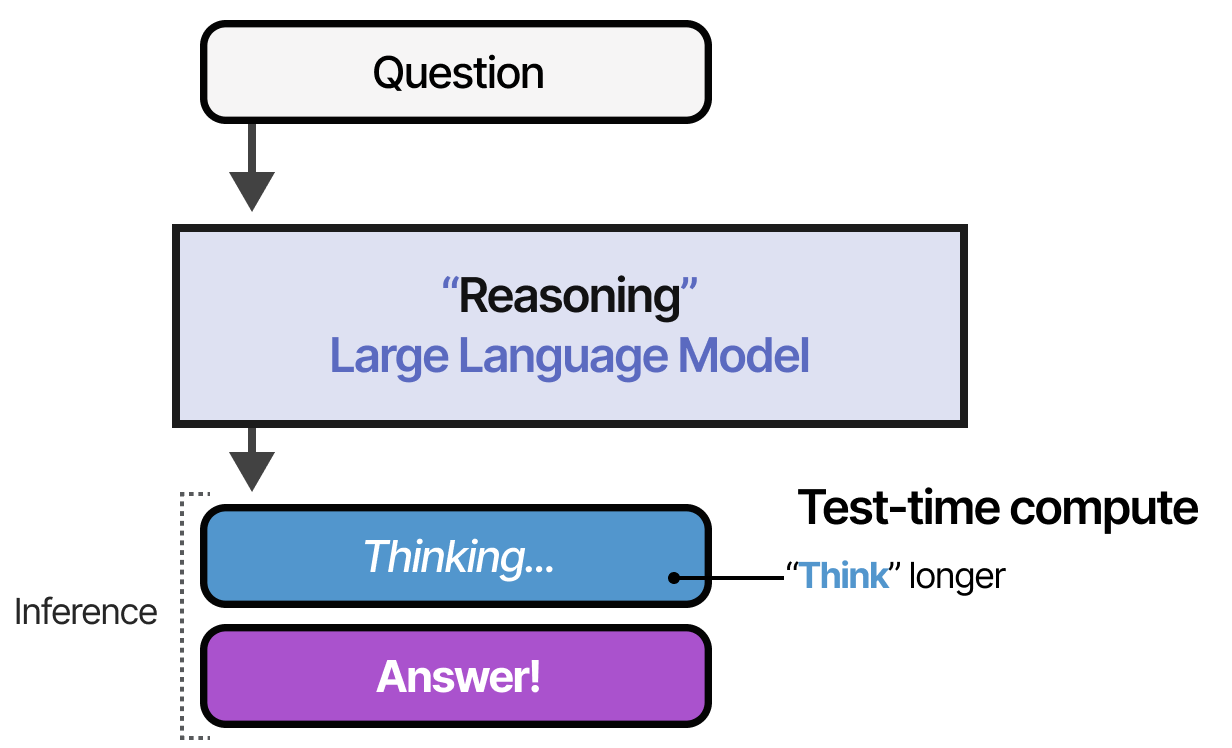
\includegraphics[width=0.7\linewidth,keepaspectratio]{llm246}
		
		$---$
		
        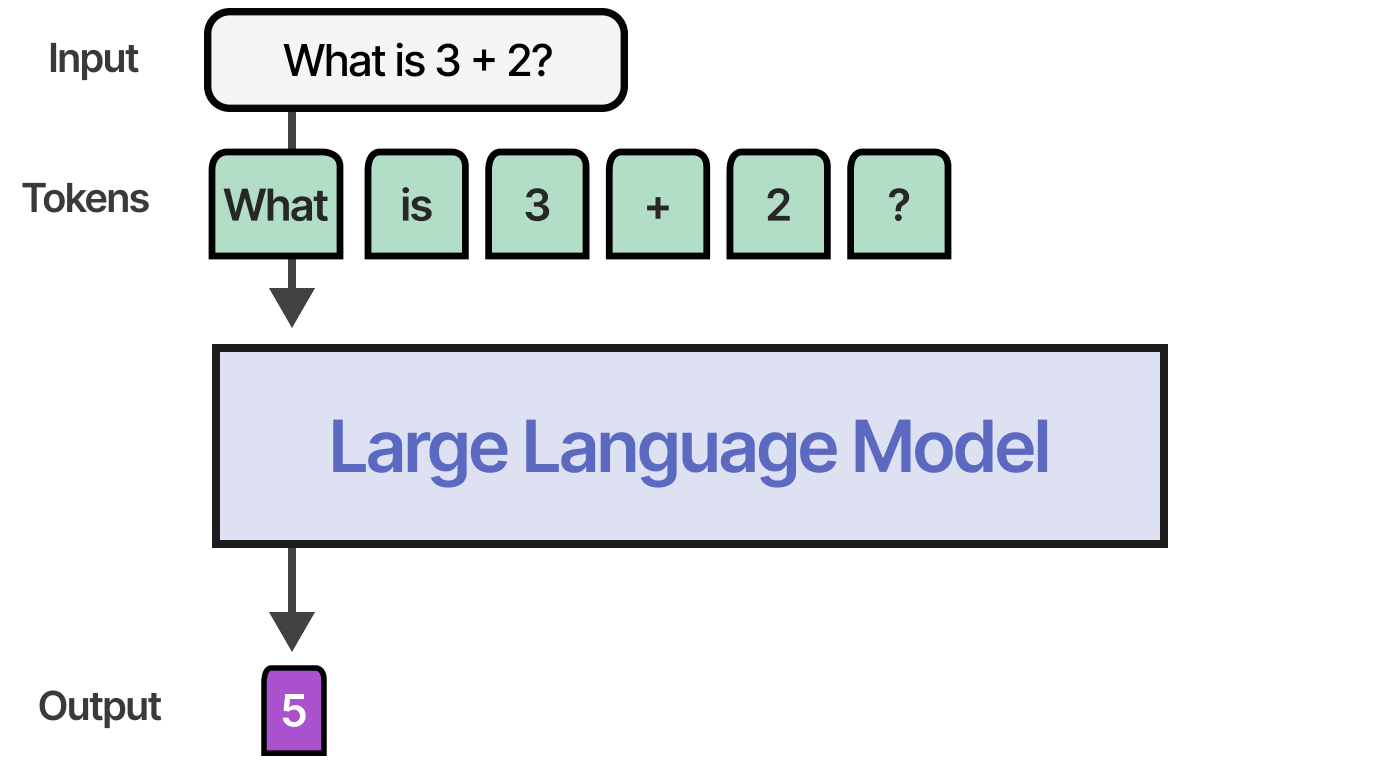
\includegraphics[width=0.7\linewidth,keepaspectratio]{llm247}
		
		{\tiny (Ref: A Visual Guide to Reasoning LLMs - Maarten Grootendorst)}
		
        \end{center}    
    \end{column}
  \end{columns}
\end{frame}

%%%%%%%%%%%%%%%%%%%%%%%%%%%%%%%%%%%%%%%%%%%%%%%%%%%%%%%%%%%
\begin{frame}[fragile]\frametitle{What is Test-Time Compute?}
\begin{columns}
    \begin{column}[T]{0.5\linewidth}
        \begin{center}
        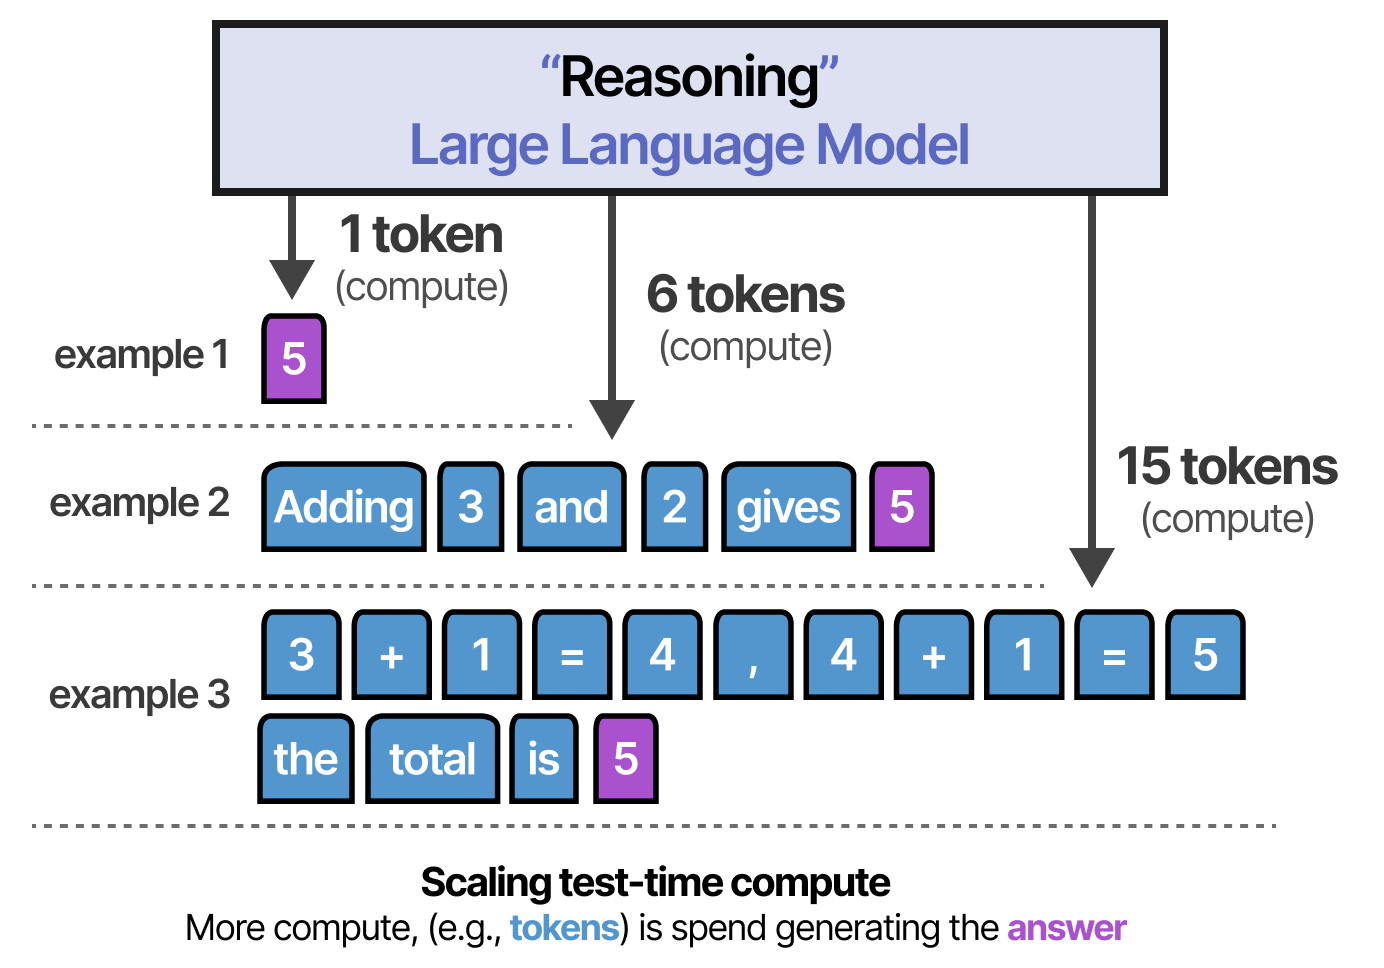
\includegraphics[width=\linewidth,keepaspectratio]{llm248}
		
		{\tiny (Ref: A Visual Guide to Reasoning LLMs - Maarten Grootendorst)}
		
        \end{center}  
    \end{column}
    \begin{column}[T]{0.5\linewidth}
        \begin{center}
        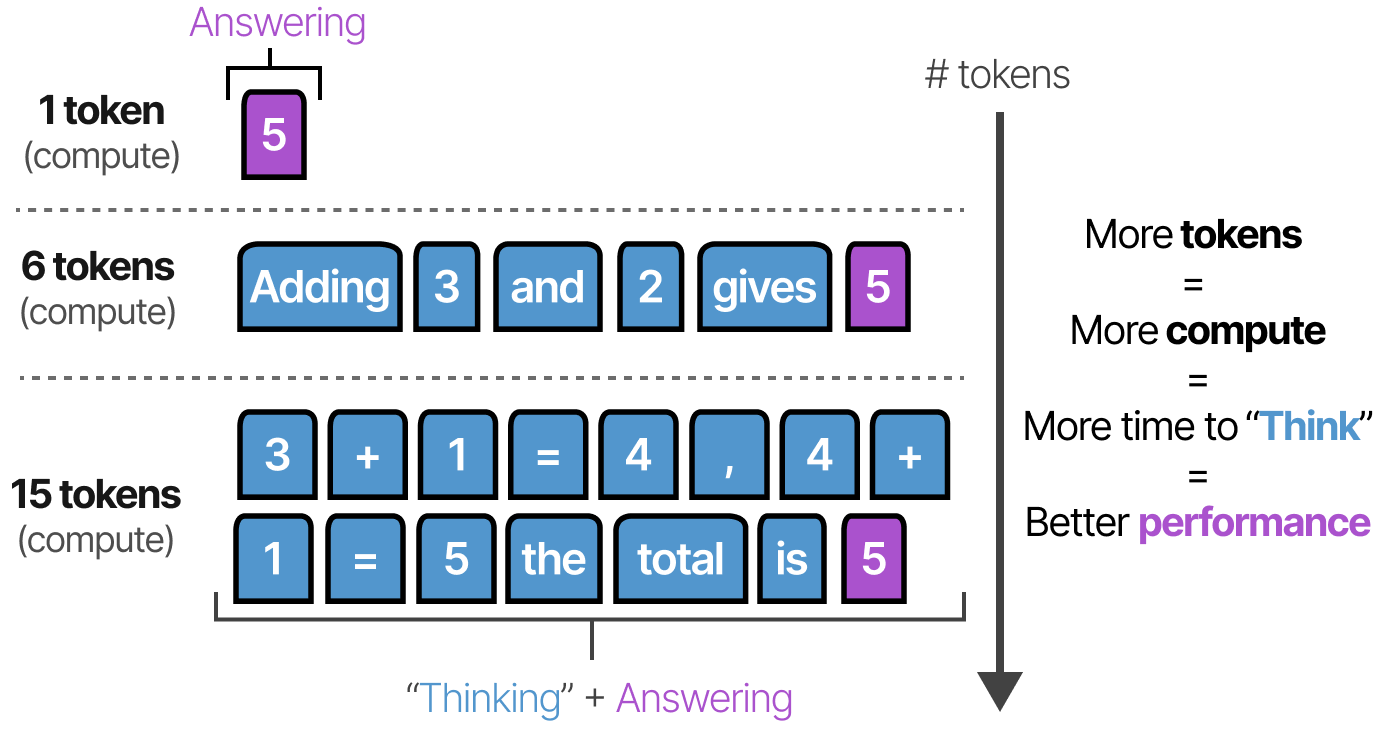
\includegraphics[width=\linewidth,keepaspectratio]{llm249}
		
		{\tiny (Ref: A Visual Guide to Reasoning LLMs - Maarten Grootendorst)}
		
        \end{center}    
    \end{column}
  \end{columns}
\end{frame}

%%%%%%%%%%%%%%%%%%%%%%%%%%%%%%%%%%%%%%%%%%%%%%%%%%%%%%%%%%%
\begin{frame}[fragile]\frametitle{Test-Time Compute Scaling Laws}

      \begin{itemize}
        \item Scaling laws for test-time compute are an emerging field.
        \item OpenAI suggests test-time compute follows similar laws to training.
        \item Shift in focus toward reasoning and inference-stage compute.
        \item “Scaling Scaling Laws with Board Games” validates this trend.
        \item Test-time and train-time compute are strongly related.
        \item Minimum compute thresholds were found for target performance.
      \end{itemize}

        \begin{center}
        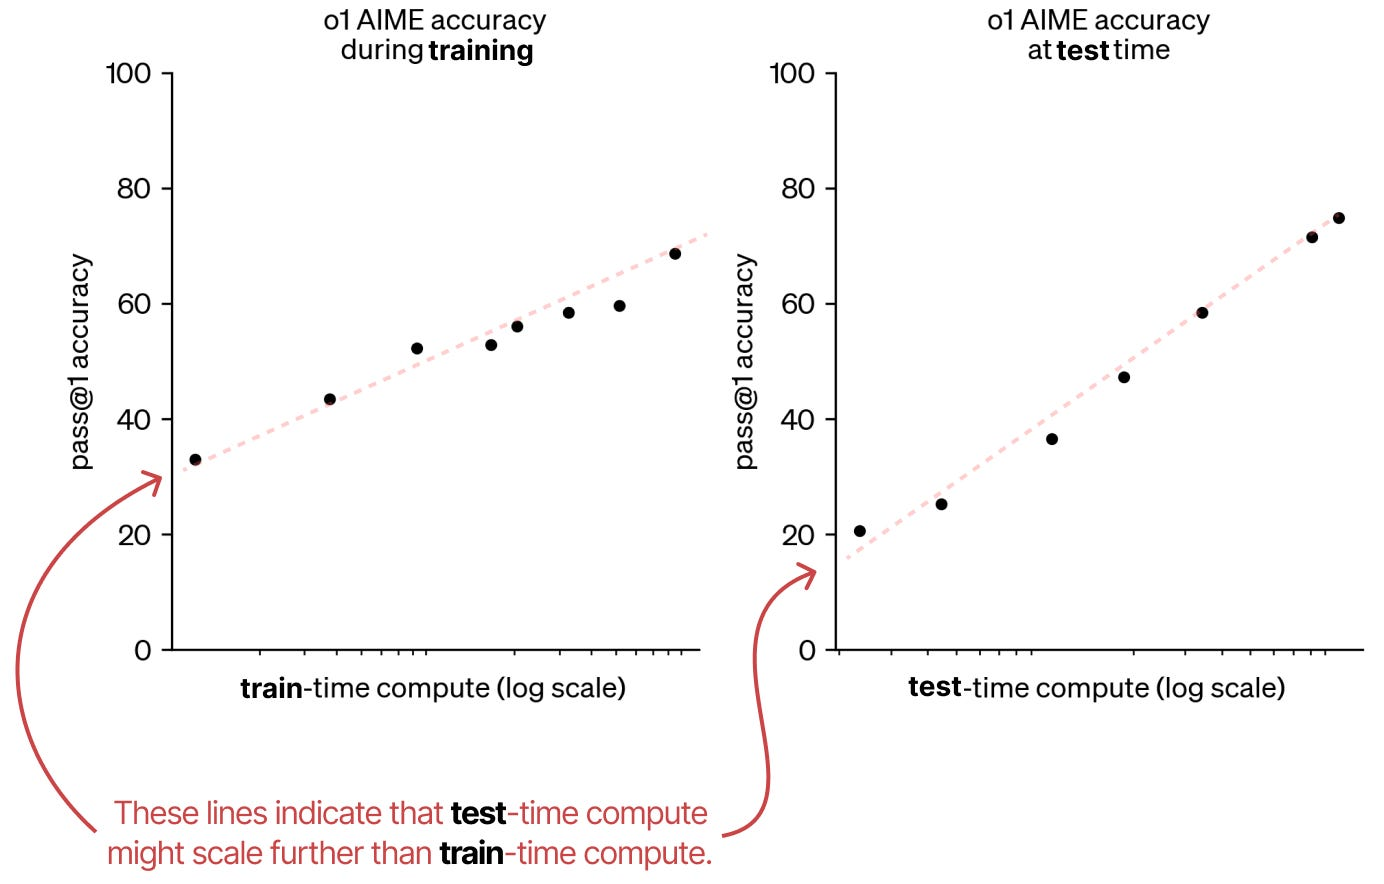
\includegraphics[width=0.6\linewidth,keepaspectratio]{llm250}
		
		{\tiny (Ref: A Visual Guide to Reasoning LLMs - Maarten Grootendorst)}
		
        \end{center}    

\end{frame}

%%%%%%%%%%%%%%%%%%%%%%%%%%%%%%%%%%%%%%%%%%%%%%%%%%%%%%%%%%%
\begin{frame}[fragile]\frametitle{Paradigm Shift in Compute Strategy}
\begin{columns}
    \begin{column}[T]{0.5\linewidth}
      \begin{itemize}
        \item Traditional focus was on train-time compute for performance.
        \item Reasoning models mark a shift toward test-time compute.
        \item Future models may balance training and inference budgets.
        \item Test-time compute may scale with token generation length.
        \item Enables models to dynamically adjust reasoning effort.
        \item DeepSeek-R1 explores this inference scaling paradigm further.
      \end{itemize}
    \end{column}
    \begin{column}[T]{0.5\linewidth}
        \begin{center}
        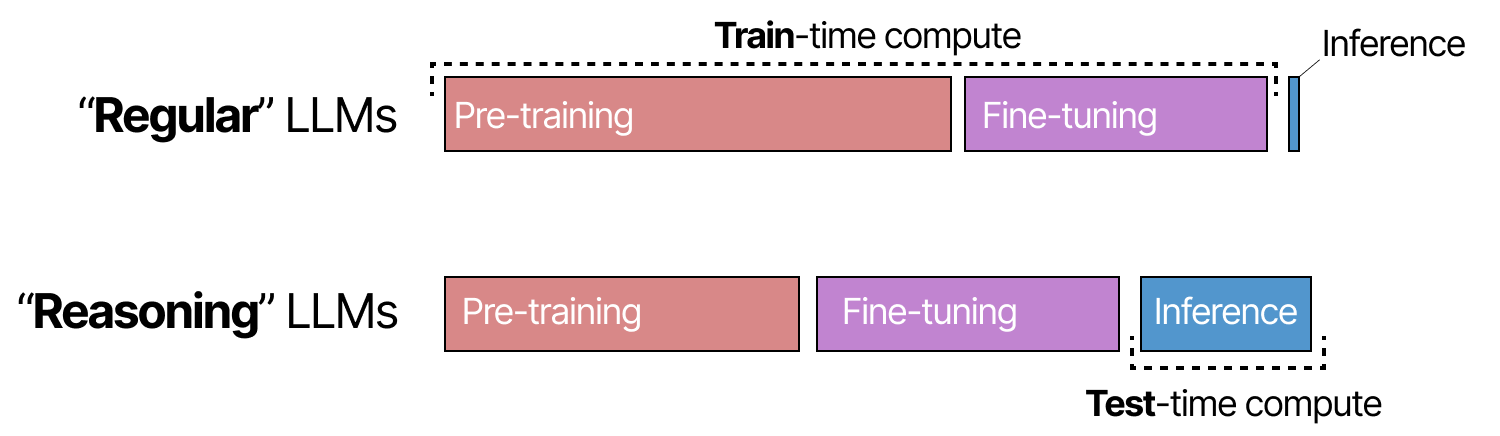
\includegraphics[width=\linewidth,keepaspectratio]{llm251}
		
		$---$
		
        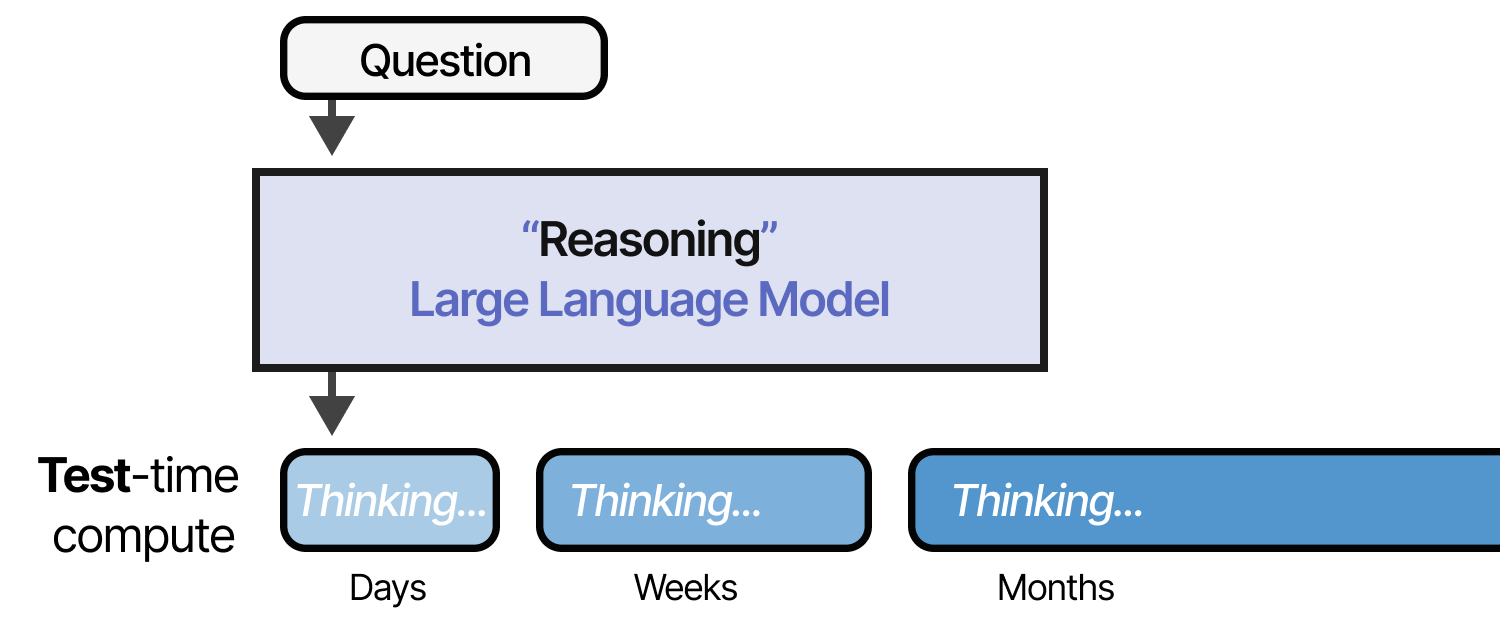
\includegraphics[width=\linewidth,keepaspectratio]{llm252}
		
		{\tiny (Ref: A Visual Guide to Reasoning LLMs - Maarten Grootendorst)}
		
        \end{center}    
    \end{column}
  \end{columns}
\end{frame}



%%%%%%%%%%%%%%%%%%%%%%%%%%%%%%%%%%%%%%%%%%%%%%%%%%%%%%%%%%%%%%%%%%%%%%%%%%%%%%%%%%
\begin{frame}[fragile]{Training: Existing: ChatGPT}
    \begin{itemize}
        \item Pretraining 
        \item Supervised Finetuning (SFT)
        \item Reinforcement Learning through Human Feedback (RLHF)
    \end{itemize}
\end{frame}

%%%%%%%%%%%%%%%%%%%%%%%%%%%%%%%%%%%%%%%%%%%%%%%%%%%%%%%%%%%%%%%%%%%%%%%%%%%%%%%%%%
\begin{frame}[fragile]{Inference}

Inference Time Strategies to build Reasoning Capabilities 

    \begin{itemize}
        \item  Chain of Thought: Long CoT allows LLMs to generate more tokens and multiple outputs thus spending more computation power on a problem during inference. 
        \item  With Long Chain of Thought (LongCoT) prompting LLMs is made to generate a series of intermediate reasoning steps before giving a final answer. 
        \item  The prompt ``Let's think this through step by step'' enables reasoning.
    \end{itemize}
\end{frame}


%%%%%%%%%%%%%%%%%%%%%%%%%%%%%%%%%%%%%%%%%%%%%%%%%%%%%%%%%%%%%%%%%%%%%%%%%%%%%%%%%%
\begin{frame}[fragile]\frametitle{Chain of Thoughts}
		\begin{center}
		\includegraphics[width=\linewidth,keepaspectratio]{promptengg25}
		\end{center}

\end{frame}


%%%%%%%%%%%%%%%%%%%%%%%%%%%%%%%%%%%%%%%%%%%%%%%%%%%%%%%%%%%%%%%%%%%%%%%%%%%%%%%%%%
\begin{frame}[fragile]{Long vs Standard CoT}


    \begin{itemize}
        \item  standard CoT is short and human-readable, a long CoT is several thousand tokens long  and not very human readable. 
		\item  long and complex reasoning trace behaviors
    \end{itemize}
\end{frame}

%%%%%%%%%%%%%%%%%%%%%%%%%%%%%%%%%%%%%%%%%%%%%%%%%%%%%%%%%%%%%%%%%%%%%%%%%%%%%%%%%%
\begin{frame}[fragile]{Parallel Decoding}


    \begin{itemize}
        \item   Instead of generating a single output with LLM, it generates multiple 
outputs and aggregates these outputs to form a single, final answer. 
    \end{itemize}
\end{frame}

%%%%%%%%%%%%%%%%%%%%%%%%%%%%%%%%%%%%%%%%%%%%%%%%%%%%%%%%%%%%%%%%%%%%%%%%%%%%%%%%%%
\begin{frame}[fragile]{AI Planning}


    \begin{itemize}
        \item AI planning is the search for a sequence of good actions to take to 
achieve a goal (maximize a reward)
\item  Classical AI Planning: solves problems by searching for an action sequence that 
transforms an initial state into a goal state. However, it depends on a correct action models, 
it may not be appropriate for LLMs
\item Reinforcement Learning AI Planning: 
	    \begin{itemize}
        \item to learn a correct sequence of decisions to 
take by interacting with an environment and receiving feedback in the 
form of rewards. 
		\item Over time, the agent learns a policy that maximizes cumulative reward 
(generates best LLM output).  
		\item DeepSeek demonstrated that reinforcement learning can drive complex reasoning improvements in AI without requiring vast supervised datasets.
		\end{itemize}

    \end{itemize}
\end{frame}

%%%%%%%%%%%%%%%%%%%%%%%%%%%%%%%%%%%%%%%%%%%%%%%%%%%%%%%%%%%%%%%%%%%%%%%%%%%%%%%%%%
\begin{frame}[fragile]\frametitle{What is Reinforcement Learning?}
		\begin{center}
		\includegraphics[width=\linewidth,keepaspectratio]{rl1}
		\end{center}

\end{frame}


%%%%%%%%%%%%%%%%%%%%%%%%%%%%%%%%%%%%%%%%%%%%%%%%%%%%%%%%%%%%%%%%%%%%%%%%%%%%%%%%%%
\begin{frame}[fragile]{Use of RL in LLMs}


    \begin{itemize}
        \item  RLHF to fine tune a model
		\item RL to train an AI agent that uses an LLM as part of its decision process.
		\item An LLM agent acting in a simulated environment (say, a text-based 
game or a web navigation task) can be improved via RL by trying actions, 
seeing outcomes, and learning a policy. 
		\item However, pure RL can be sample-inefficient (requiring many trials) and 
lacks guarantees of optimality. Modern techniques like model-based RL 
explicitly learn a model of the environment and plan within it, blending 
classical planning ideas with reinforcement learning.
    \end{itemize}
\end{frame}


%%%%%%%%%%%%%%%%%%%%%%%%%%%%%%%%%%%%%%%%%%%%%%%%%%%%%%%%%%%%%%%%%%%%%%%%%%%%%%%%%%
\begin{frame}[fragile]{To Enhance Reasoning}


    \begin{itemize}
        \item  Chain-of-Thought (CoT) Prompting and Integration
        \item  Enhanced RLHF Integration
        \item  Deliberative Alignment
        \item  Train on Math and Code Combined to  Enhance Model Reasoning
        \item  Reinforcement Learning-Based Reasoning
        \item  Distillation of Large Model Reasoning into Smaller Models
    \end{itemize}
\end{frame}
